\documentclass[]{article}

\usepackage{cite} % Make references as [1-4], not [1,2,3,4]
\usepackage{url}  % Formatting web addresses 
\usepackage{ifthen}  % Conditional
\usepackage{multicol}   %Columns
\usepackage[utf8]{inputenc} %unicode support
\usepackage[pdftex]{graphicx}	
\usepackage{verbatim}
\usepackage{booktabs}
\usepackage{xr}
\usepackage{hyperref}

\begin{document}

\title{Supplementery Information}
%\author{Daniel Murrell}
\maketitle

% Table generated by Excel2LaTeX from sheet 'results.csv'
\begin{table}[htbp]
  \centering
  \caption{Comparison to existing methods.}
    \begin{tabular}{rrrr}
    \toprule
    Model & PKKB  & Martel & Average \\
    \midrule
    smlogp & 0.859 & 1.222 & 1.040 \\
    spluslogp & 0.938 & 1.392 & 1.165 \\
    p.crippen & 1.196 & 1.172 & 1.184 \\
    alogps & 0.863 & 1.546 & 1.205 \\
    alogp & 1.292 & 1.281 & 1.287 \\
    mlogp & 0.794 & 2.053 & 1.423 \\
    xlogp3 & 1.741 & 1.177 & 1.459 \\
    p.xlogp & 1.569 & 1.393 & 1.481 \\
    milogp & 2.479 & 1.176 & 1.828 \\
    am    & 2.511 & 1.187 & 1.849 \\
    p.mlogp & 2.028 & 1.704 & 1.866 \\
    clogp & 2.241 & 1.560 & 1.900 \\
    p.alogp & 3.566 & 4.338 & 3.952 \\
    \bottomrule
    \end{tabular}%
  \label{tab:external_comparison}%
\end{table}%

\begin{table}[htbp]\footnotesize
  \centering
  \caption{Descriptors used in model training.}
    \begin{tabular}{rrrr}
    \toprule
   %\hline
    nAcid & nAromBond & nH    & nC \\
    %\midrule
    nN    & nS    & nF    & nCl \\
    nX    & ATSc1 & ATSc2 & ATSc3 \\
    ATSc4 & ATSc5 & ATSm1 & ATSm3 \\
    ATSm4 & ATSm5 & nBase & BCUTw.1l \\
    BCUTw.1h & BCUTc.1l & BCUTc.1h & BCUTp.1l \\
    BCUTp.1h & nBondsD & nBondsD2 & nBondsM \\
    bpol  & C1SP2 & C2SP2 & C3SP2 \\
    C1SP3 & C2SP3 & C3SP3 & C4SP3 \\
    SCH.5 & SCH.6 & SCH.7 & VCH.3 \\
    VCH.4 & VCH.5 & VCH.6 & VCH.7 \\
    SC.3  & SC.4  & SC.5  & SC.6 \\
    VC.3  & VC.4  & VC.5  & VC.6 \\
    SPC.6 & VPC.6 & SP.7  & VP.7 \\
    CrippenLogP & nHBa  & nwHBa & nHBint2 \\
    nHBint3 & nHBint4 & nHBint5 & nHBint6 \\
    nHBint7 & nHBint8 & nHBint9 & nHBint10 \\
    nHsOH & nHdNH & nHaaNH & nHCHnX \\
    nHCsats & nHCsatu & nHAvin & nssCH2 \\
    nsssCH & ntsC  & ndssC & naasC \\
    naaaC & nssssC & ndsN  & naaN \\
    nsssN & naasN & ndO   & nssO \\
    naaO  & nssS  & nddssS & SHBd \\
    SHBa  & SwHBa & SHBint2 & SHBint3 \\
    SHBint4 & SHBint5 & SHBint6 & SHBint7 \\
    SHBint8 & SHBint9 & SHsOH & SHssNH \\
    SHdsCH & SHaaCH & SHCsats & SsCH3 \\
    SssCH2 & SdsCH & SsssCH & SdssC \\
    SaasC & SssssC & SsNH2 & SssNH \\
    SsssN & minHBd & minHBa & minwHBa \\
    minHBint2 & minHBint3 & minHBint4 & minHBint5 \\
    minHBint6 & minHBint7 & minHBint8 & minHBint9 \\
    minHsOH & minHssNH & minHdsCH & minHaaCH \\
    minHCsats & minHCsatu & minHother & minsCH3 \\
    minssCH2 & mindsCH & minaaCH & minsssCH \\
    mindssC & minaasC & minssssC & minssNH \\
    mindsN & minaaN & minsssN & minsOH \\
    mindO & minssO & minsCl & maxHBa \\
    maxwHBa & maxHBint2 & maxHBint3 & maxHBint4 \\
    maxHBint5 & maxHBint6 & maxHBint7 & maxHBint8 \\
    maxHBint9 & maxHCsats & maxssCH2 & maxsssCH \\
    maxdssC & maxaasC & sumI  & hmax \\
    gmax  & hmin  & gmin  & ETA\_AlphaP \\
    ETA\_dAlpha\_B & ETA\_Epsilon\_1 & ETA\_Epsilon\_2 & ETA\_Epsilon\_4 \\
    ETA\_Epsilon\_5 & ETA\_dEpsilon\_B & ETA\_dEpsilon\_D & ETA\_Psi\_1 \\
    ETA\_dPsi\_A & ETA\_Shape\_P & ETA\_Shape\_Y & ETA\_Shape\_X \\
    ETA\_BetaP & ETA\_BetaP\_s & ETA\_dBeta & ETA\_Beta\_ns\_d \\
    ETA\_BetaP\_ns\_d & ETA\_EtaP & ETA\_EtaP\_F & ETA\_Eta\_F\_L \\
    ETA\_EtaP\_F\_L & ETA\_Eta\_B & ETA\_EtaP\_B & ETA\_Eta\_B\_RC \\
    ETA\_EtaP\_B\_RC & FMF   & fragC & nHBAcc \\
    nHBAcc3 & nHBAcc\_Lipinski & nHBDon\_Lipinski & HybRatio \\
    Kier2 & Kier3 & nAtomLC & nAtomP \\
    nAtomLAC & MDEC.11 & MDEC.12 & MDEC.13 \\
    MDEC.22 & MDEC.23 & MDEC.33 & MDEO.11 \\
    MDEO.12 & MDEN.22 & MDEN.23 & MLFER\_A \\
    MLFER\_BH & MLFER\_S & MLFER\_E & MLFER\_L \\
    PetitjeanNumber & nRing & nFRing & nF9Ring \\
    nF10Ring & nFG12Ring & nTRing & nT5Ring \\
    nT6Ring & nRotB & LipinskiFailures & TopoPSA \\
    VAdjMat & WTPT.2 & WTPT.3 & WTPT.4 \\
    WPATH &       &       &  \\
    \bottomrule
    \hline
    \end{tabular}%
  \label{tab:descriptors}%
\end{table}%

% GRID SEARCH FIGURE
\begin{figure}[ht]
  \centering
  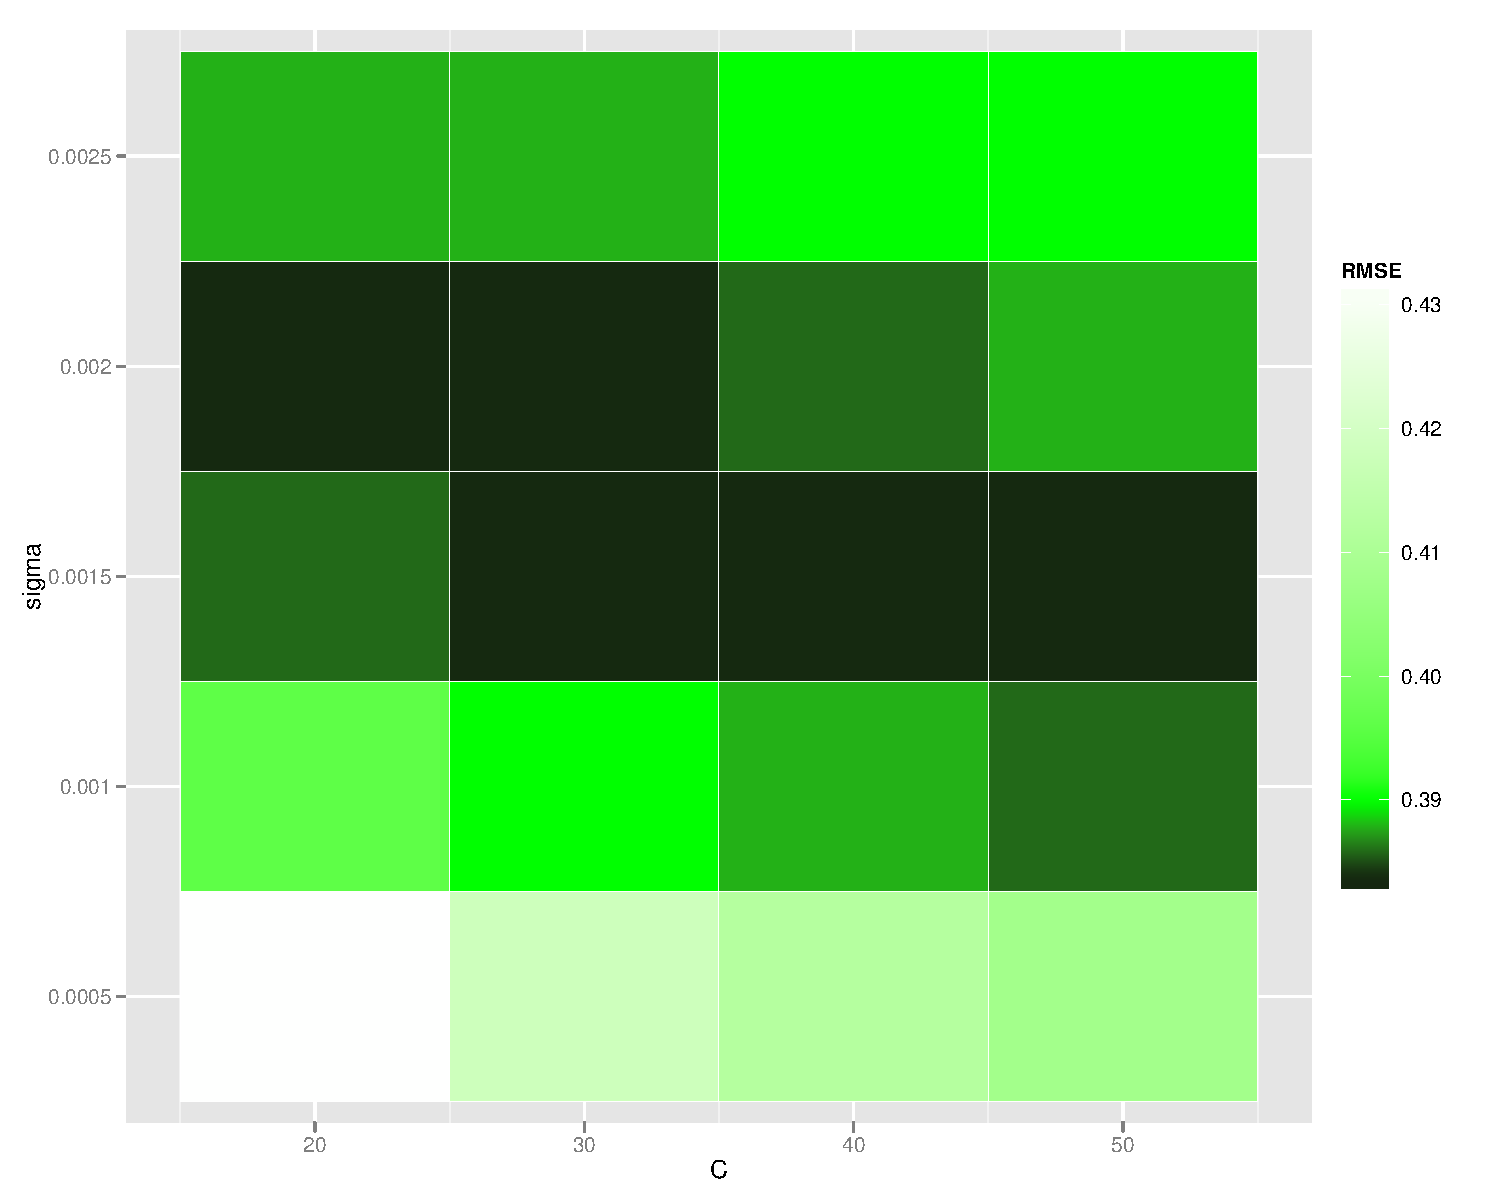
\includegraphics[width=0.95\textwidth]{./figures_si/grid_search.pdf}
  \caption{Grid search over a narrow parameter space. $\sigma$ and Cost
    hyperparameters are optimised by comparing the model's mean RMSE over the 5
    validation sets.}
  \label{fig:grid_search}
\end{figure}

% PCA FIGURE
%\begin{figure}[ht]
%  \centering
%  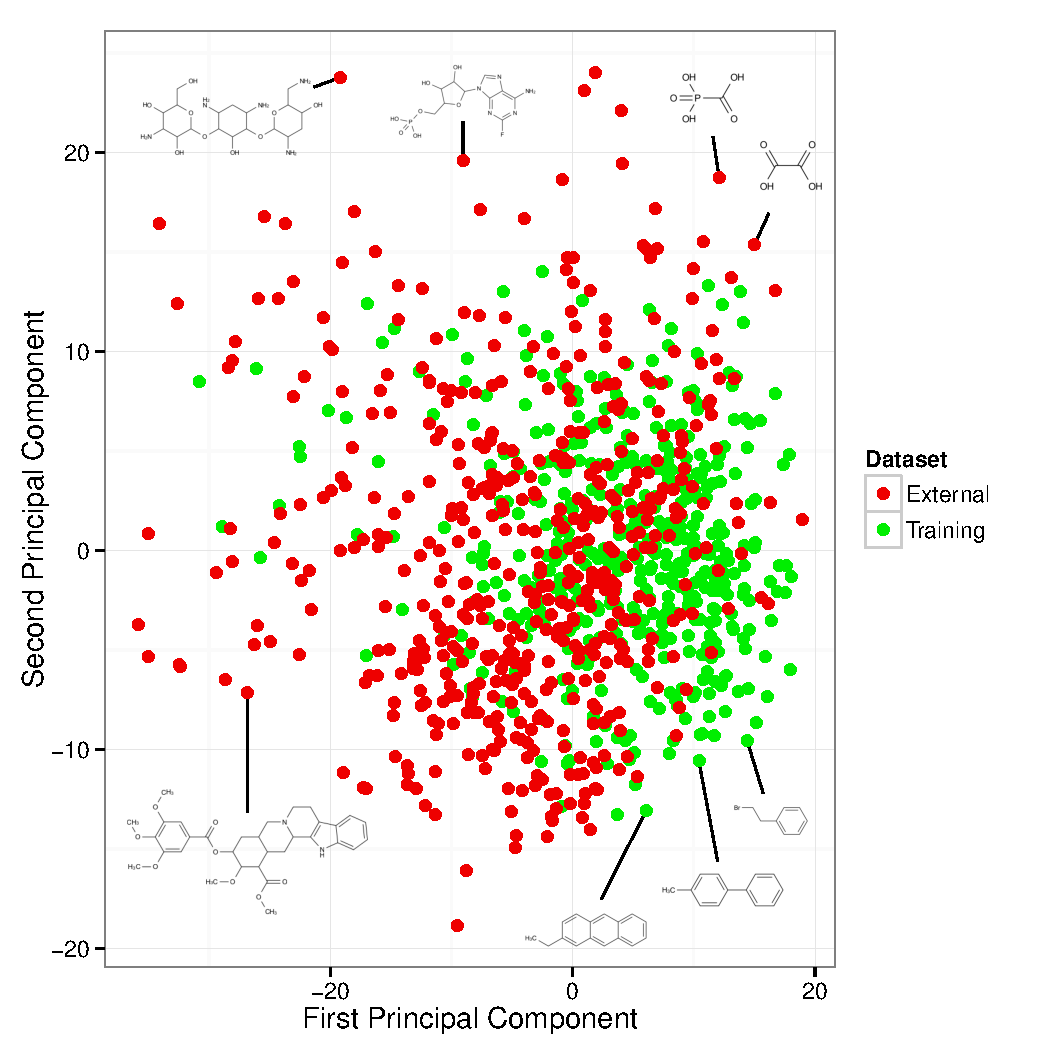
\includegraphics[width=0.95\textwidth]{./figures_si/pca.pdf}
%  \caption{PCA of training and external test sets. Training set size is cut down to that of external set size in a random fashion TBD reword.}
%  \label{fig:grid_search}
%\end{figure}

% SCATTER PLOTS
\begin{figure}[ht]
  \centering
  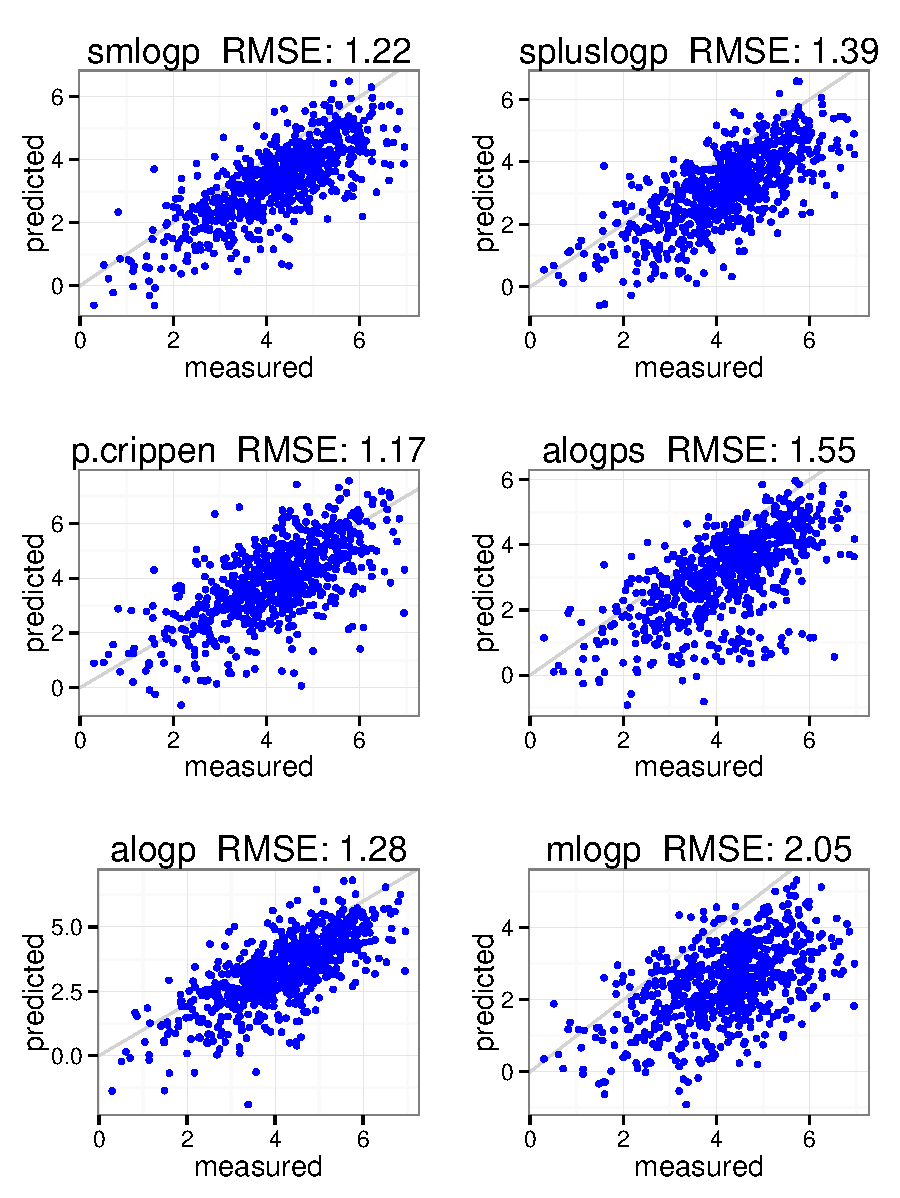
\includegraphics[width=0.95\textwidth]{./figures_si/martel_scatter_1.pdf}
  \caption{Correlation plots of the top (averaged over both external sets) 6 methods on the Martel set.}
  \label{fig:external_comparison1}
\end{figure}

\begin{figure}[ht]
  \centering
  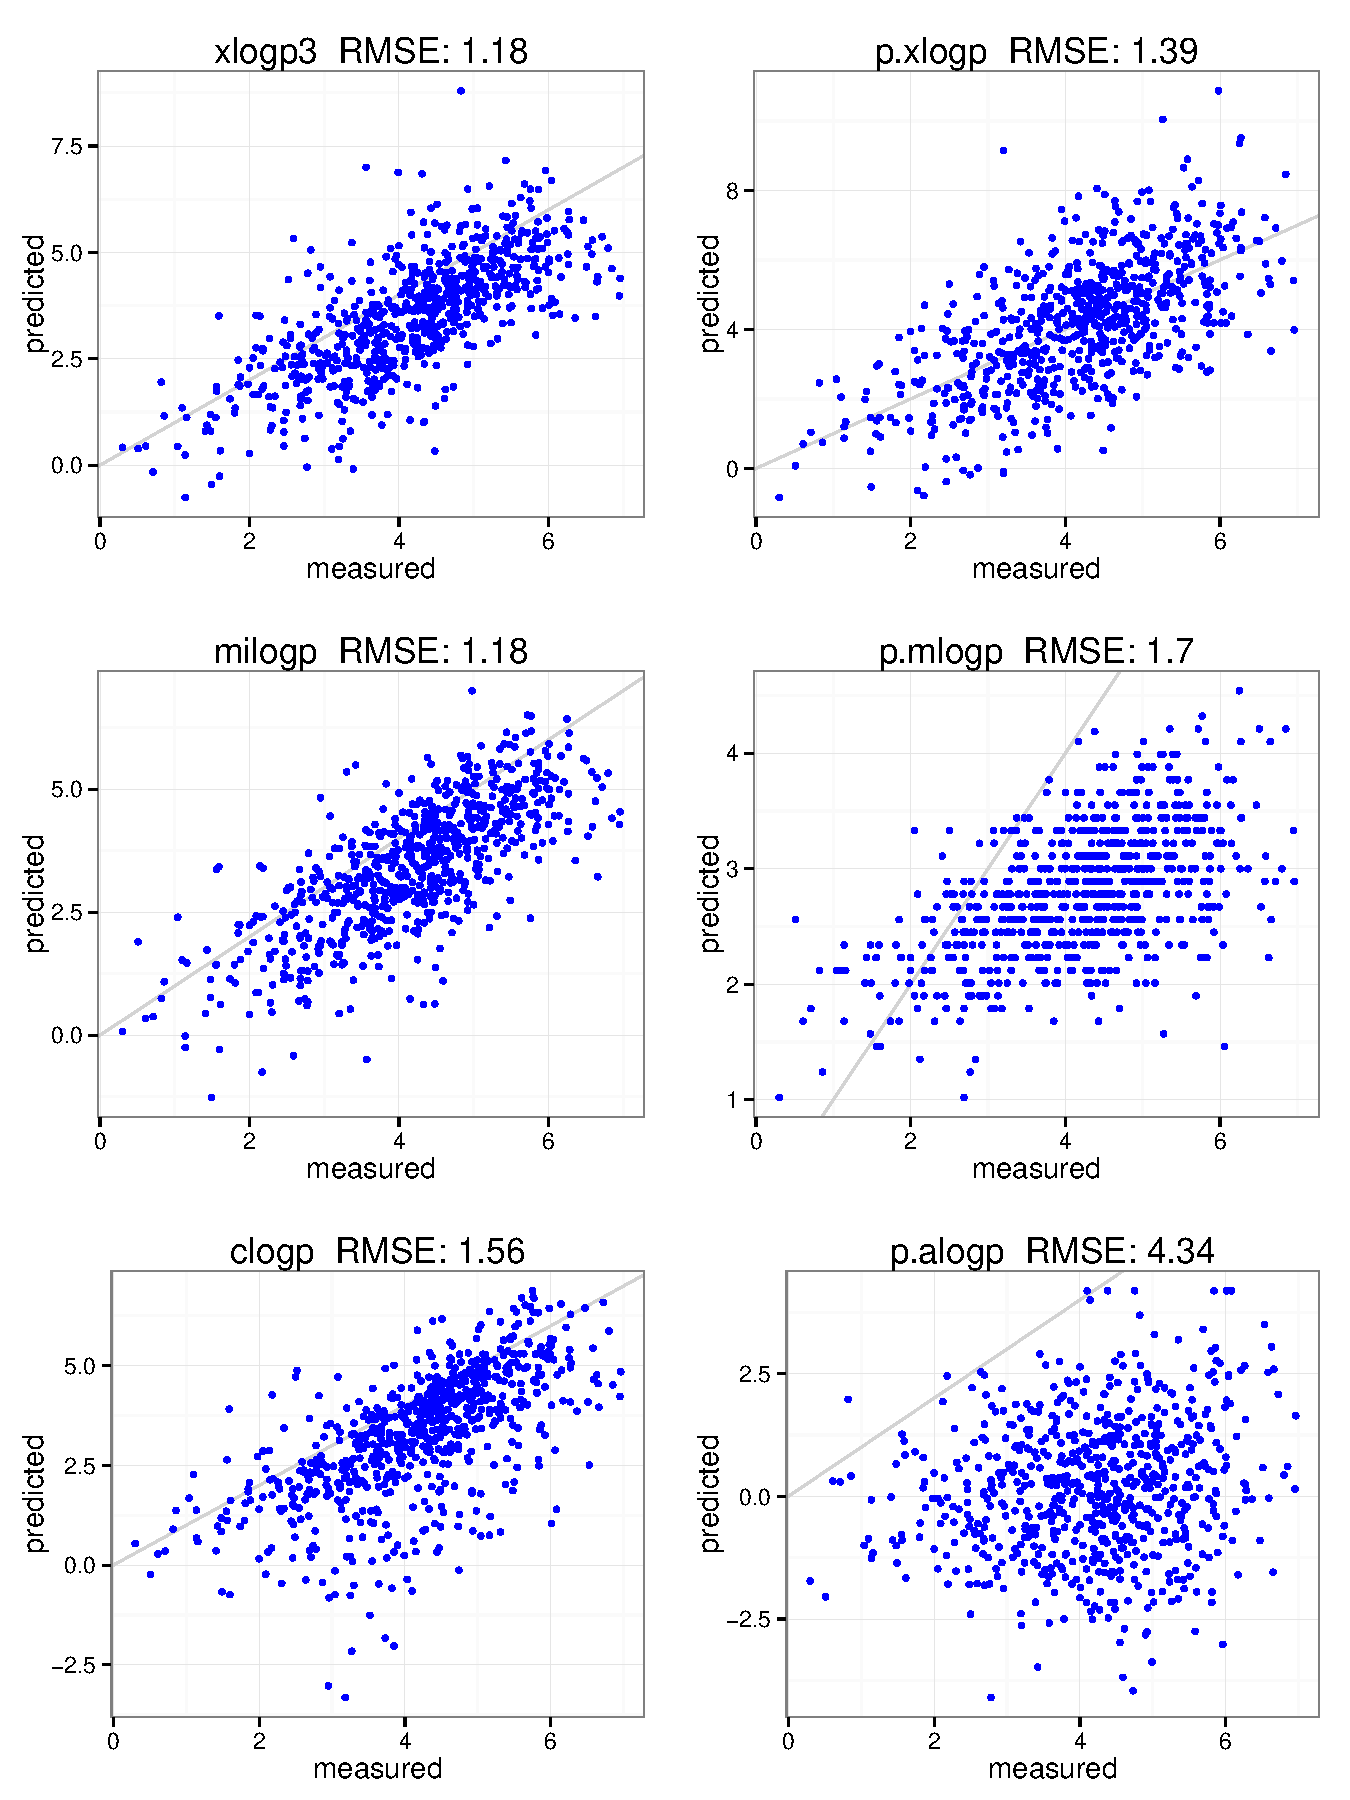
\includegraphics[width=0.95\textwidth]{./figures_si/martel_scatter_2.pdf}
  \caption{Correlation plots of the bottom (averaged over both external sets) 6 methods on the Martel set.}
  \label{fig:external_comparison2}
\end{figure}

\begin{figure}[ht]
  \centering
  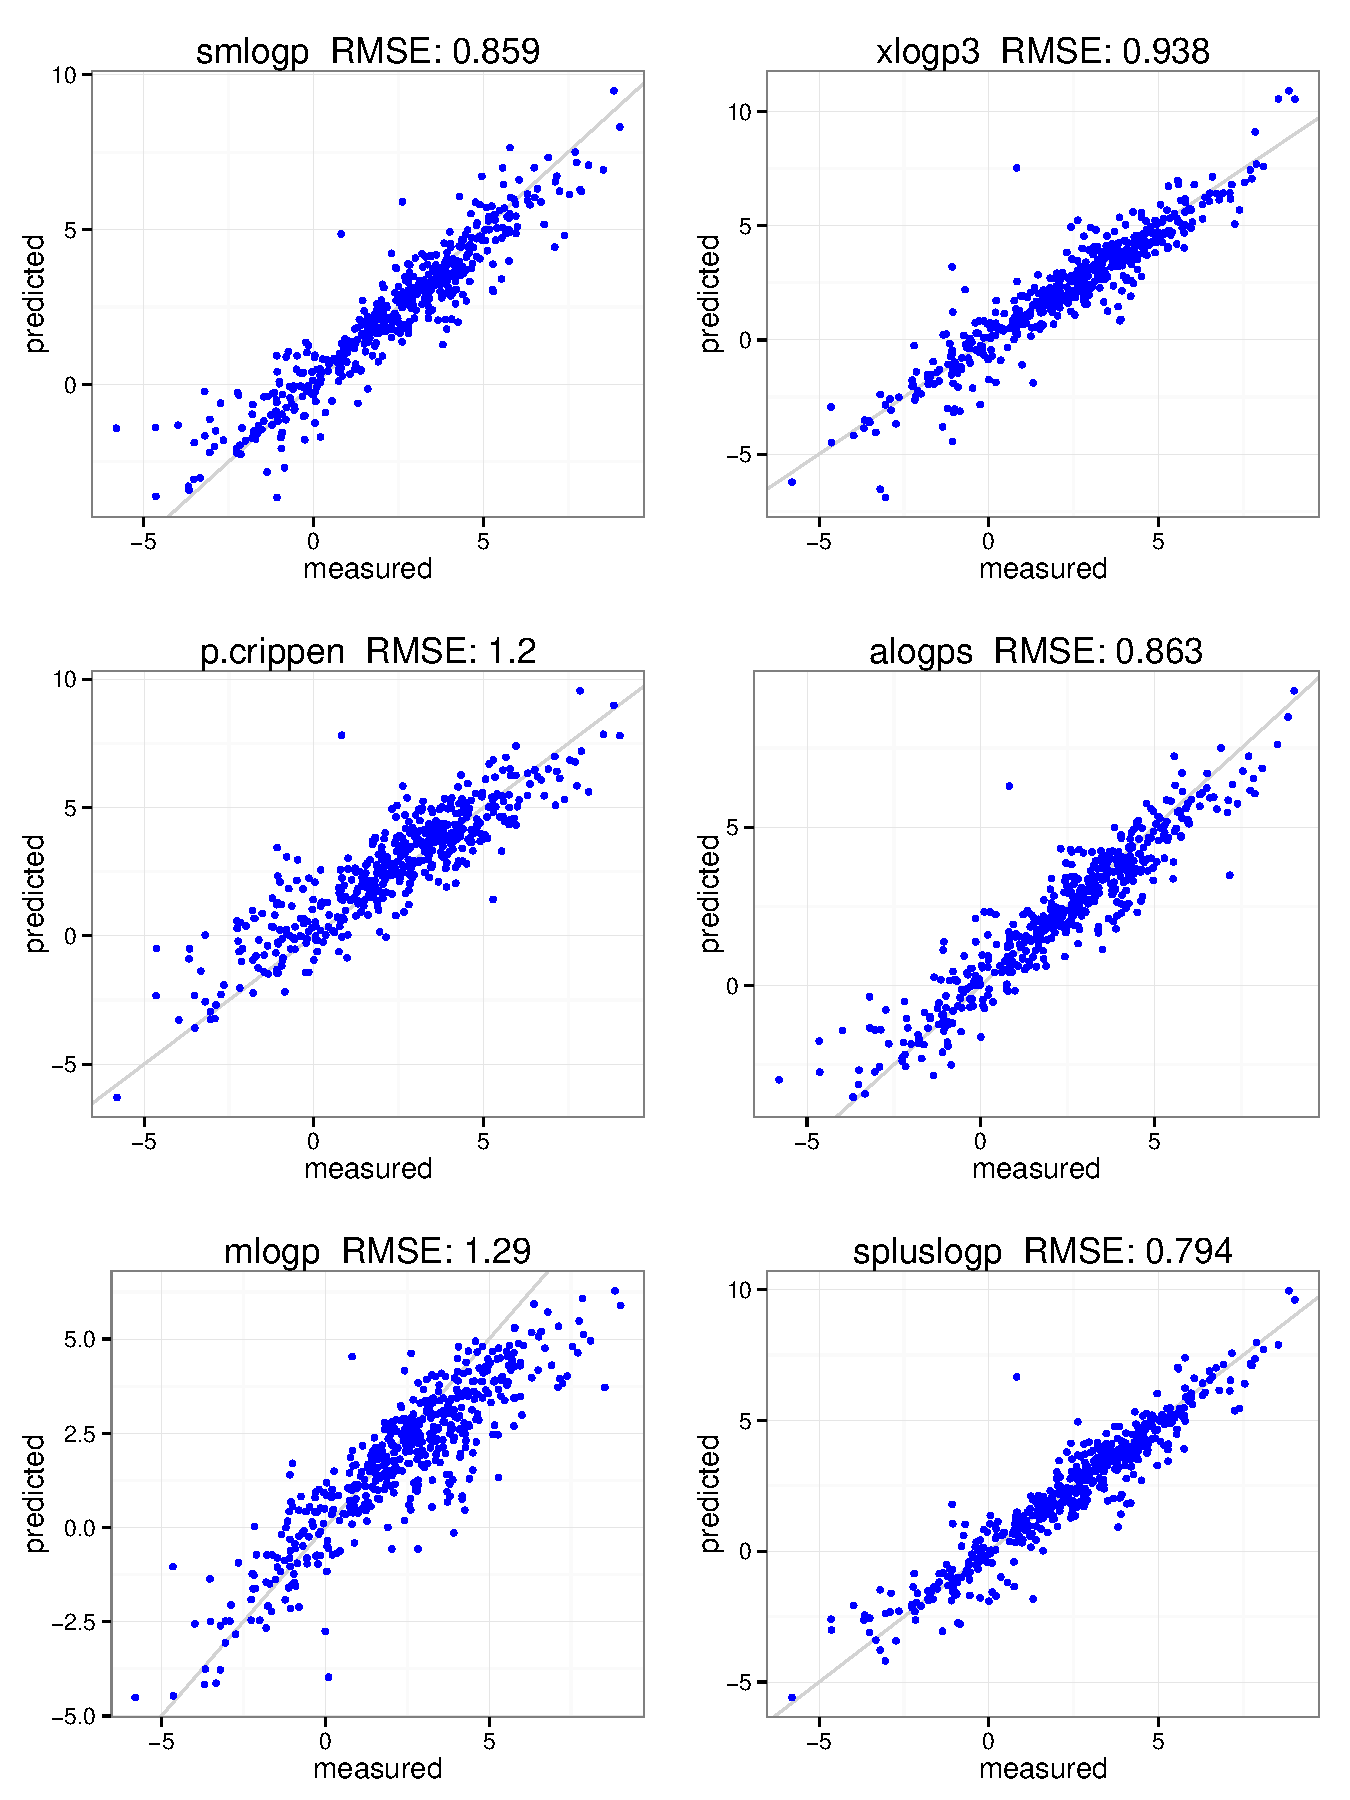
\includegraphics[width=0.95\textwidth]{./figures_si/pkkb_scatter_1.pdf}
  \caption{Correlation plots of the top (averaged over both external sets) 6 methods on the PKKB set.}
  \label{fig:external_comparison3}
\end{figure}

\begin{figure}[ht]
  \centering
  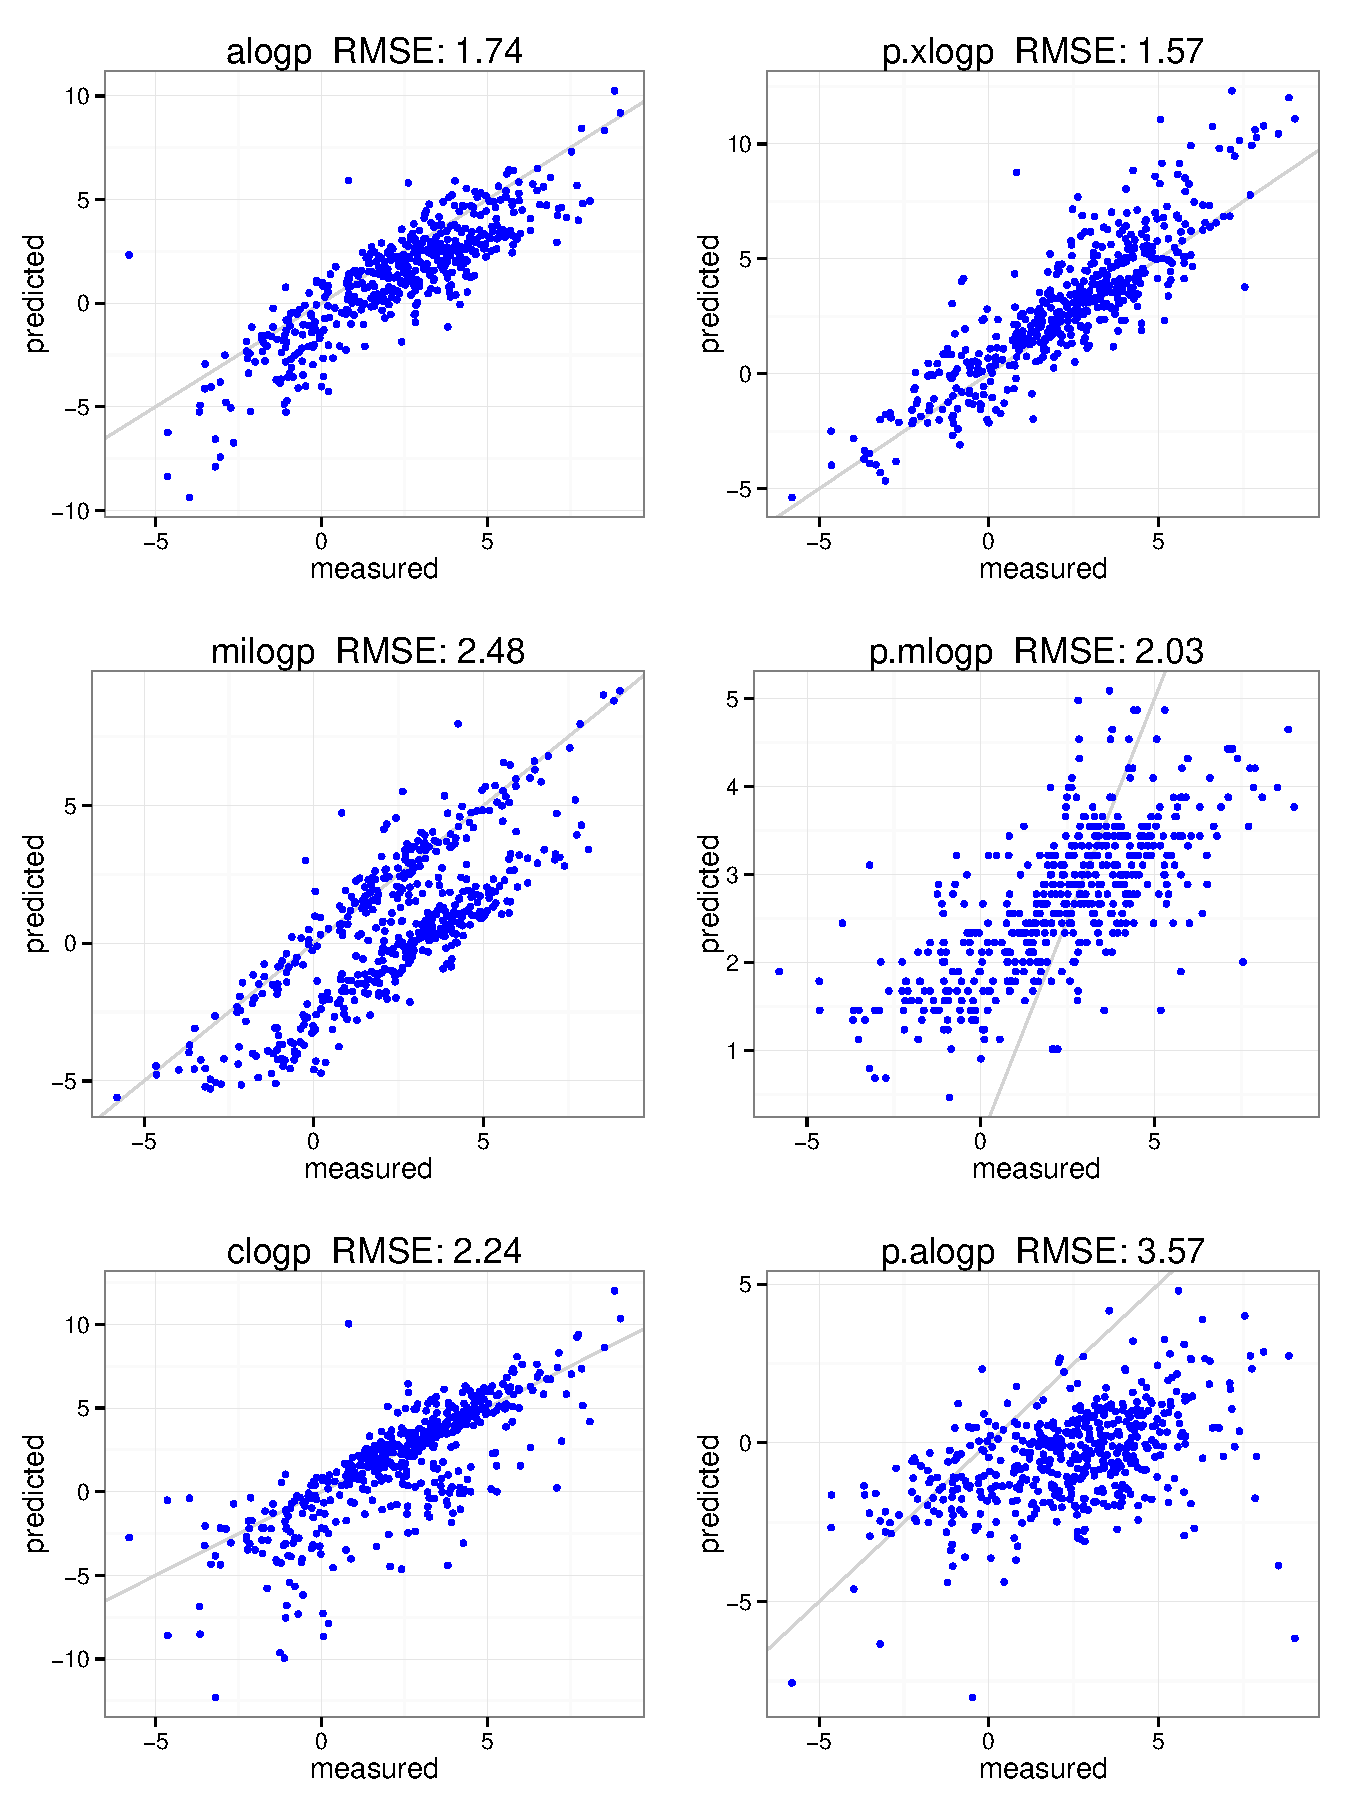
\includegraphics[width=0.95\textwidth]{./figures_si/pkkb_scatter_2.pdf}
  \caption{Correlation plots of the bottom (averaged over both external sets) 6 methods on the PKKB set.}
  \label{fig:external_comparison4}
\end{figure}

\end{document}